\label{chapter6}
\chapter{Presenting proposed profiles}

Previously defined profiles will be presented in-depth. 
In general, each profile has its use case already assigned in table \ref{tab:use_cases}.
Here, we will focus on exposing the main features, issues, and use cases. 

Data for profiles in this chapter was used from the REFIT dataset and building 2.
Data was collected from 2013-09-18 to 2015-05-28.
\section{Time ranges}
One important thing to mention is to use cases for different time ranges of load profiles.
Based on table \ref{tab:contributions} it is possible to see that most publications and \ref{tab:use_cases} use daily time range.

Generally, daily profiles are easier to build since they do not need as much data as others do.
To build a decent profile one needs enough data. 
A sufficient amount of data is the amount that covers major events.
For a daily profile, a few weeks of data is enough, weekly load profiles need a few months of data, monthly few months, and yearly few years.
And this is the main issue, there is rarely enough data to build such profiles.
Even then, usage patterns could change over a long period such as a decade.
Combining that with a smaller number of use cases for such profiles, reveals why such profiles were not looked into as much.

One more thing about time ranges that need to be mentioned are patterns that they present.
Daily profiles present daily usage and enable us to extract contextual events such as waking up, cooking, leisure time, etc.
The weekly pattern is also repetitive, and it enables us to see how appliance usage changes over the weekdays and weekends.
The monthly profile has none of the above. It is not repetitive since each day of the month can be a different day of the week, and the period is too short to capture seasonal patterns.
Alternatively, it could be presented as a week in a month, but there is no significant usage pattern to be revealed.
The yearly profile on the other hand presents the seasonal effects on usage such as increased daylight and temperature. 


\section{Per-house}

The section will be focused on per-house profiles, meaning whole building usage is presented as a single load profile.
This kind of presentation is useful for observing general activation trends in a building.
Possible use cases for per-house load profiles are grid management and energy saving.

When it comes to activation load profiles there is one issue compared to power load profiles.
To build per-house power load profiles it is possible to use the main power meter, whereas, at activation load profiles, sub-meter data is needed.
This can be solved using NILM algorithms, but they are not in a phase of practical use yet.

The daily per-house load profile is also known as the standard load profile. 
According to table \ref{tab:contributions} this is the most commonly used power profile.
Figures \ref{fig:SLPdaily2} and \ref{fig:SLPyearly2} present usage patterns on different time ranges. 
The two profiles, therefore present different contextual causes.


\begin{figure}[H]
	\begin{subfigure}{.5\textwidth}
		% \centering
		\caption{"Daily"}
		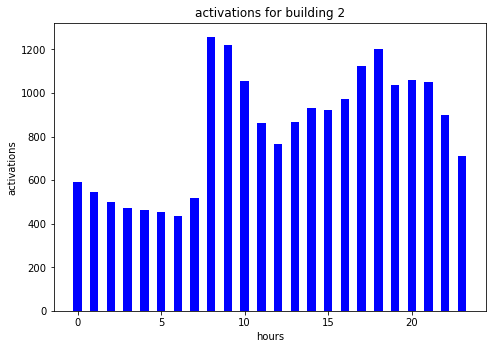
\includegraphics[width=1\linewidth]{../Figures/LPS/SLPdaily2.png}
		\label{fig:SLPdaily2}
	\end{subfigure}%
	~ 
	\begin{subfigure}{.5\textwidth}
		% \centering
		\caption{"Yearly"}
		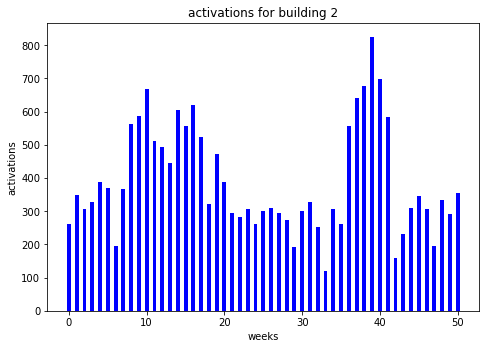
\includegraphics[width=1\linewidth]{../Figures/LPS/SLPyearly2.png}
		\label{fig:SLPyearly2}
	\end{subfigure}%
	\label{fig:SLP}
	\caption{"per-house load profiles"}
\end{figure}

\subsection{Per-house two-dimensional time}

Alternatively, it is possible to combine figures \ref{fig:SLPdaily2} and \ref{fig:SLPyearly2} and present activations as a heat map.
The result is a load profile showing more complex activation patterns.

\begin{figure}[H]
	\centering
	\caption{"Two-dimensional time per-house load profile"}
	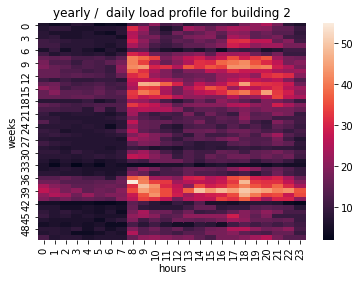
\includegraphics[width=0.7\textwidth]{../Figures/LPS/SLPHMyearly2.png}
	\label{fig:SLPHMyearly2}
\end{figure}

Previously it was mentioned that these kinds of profiles are the most applicable in grid management and energy-saving fields. 
One such example could be load shedding.
Using the Load profile above, electrical energy providers could find buildings with the least activity at that time of day.
Combining that with power data, it could disconnect the buildings with the least activity and most power consumption.

\section{Per-appliance}

Per appliance load profiles offer a look into the consumption of each appliance. 
In this case activation load profiles, this is an elemental load profile, since all other 
profiles are built on top of it. 
This also means that it is one of the most universal profiles since it can be used in all previously defined use cases.
Comparing power and activation profiles in the per-house chapter,
it was possible to see that activation-based load profile does not bring significant advantages over power-based load profiles.
In the case of per-appliance load profiles, it is possible to analyze the usage of the single appliance in greater detail

\begin{figure}[H]
	\centering
	\caption{"Daily per-appliance load profile"}
	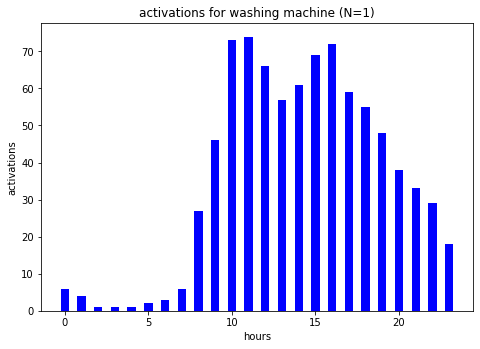
\includegraphics[width=0.7\textwidth]{../Figures/LPS/WM_daily.png}
	\label{fig:WM_daily}
\end{figure}

Another parameter that was not explicitly mentioned before, is the resolution of load profiles. 
Histograms can be presented using various resolutions or numbers of buckets.
An optimal number of buckets is a number that clearly presents the usage pattern. 
3-hour bucket size on figure \ref{fig:4hours} does a good job at presenting the appliance usage at the main parts of the day.
This offers a better contextual presentation that is easier to process using algorithms.
Parts of the day are:

\begin{figure}[H]
	\centering
	\caption{"Daily per-appliance load profile with larger buckets sizes"}
	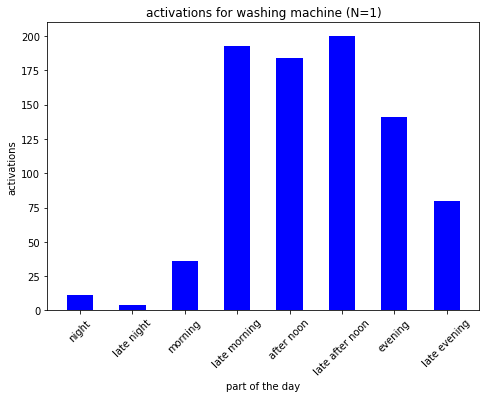
\includegraphics[width=0.7\textwidth]{../Figures/LPS/3 hours.png}
	\label{fig:4hours}
\end{figure}


While the low resolution is useful for contextual presentation,
high resolution is needed for time-sensitive applications such as elderly care,
where we have to detect an accident as soon as possible.
The hourly resolution would mean that in case of an accident system would need at least an hour to detect it.
While this is sufficient for demonstrating the capabilities, real implementation would need to use lower resolution data.

In case, dwellers have different usage patterns during the weekends, two profiles would have to be developed.
It is possible to present them both at once such as in figure \ref{fig:WM_ww_daily}. 
This is essentially a variation of the weekly Load profile that maintains high resolution.
Since there are more weekdays than weekend days, activations had to be normalized accordingly.
\begin{figure}[H]
	\centering
	\caption{"Normalized daily per-appliance with weekday and weekend load profiles"}
	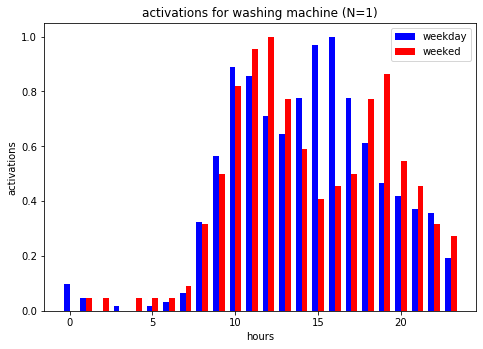
\includegraphics[width=0.7\textwidth]{../Figures/LPS/WM_ww_daily.png}
	\label{fig:WM_ww_daily}
\end{figure}

Another way to present weekly data is figure \ref{fig:WM_weekly}
This resolution offers a look into how consumption pattern changes over
the week. This is useful for applications such as grid management and energy saving.
In this particular case, it is possible to see that the user most commonly uses the washing machine on Mondays and Wednesdays.
Using a weekly weather report that would indicate high energy production on Wednesday, electricity provider could offer a low cost for energy for that day. 
This kind of presentation could also be used to detect daily anomalies.

\begin{figure}[H]
	\centering
	\caption{"Weekly per-appliance load profile"}
	\includegraphics[width=0.7\textwidth]{../Figures/LPS/WM_weekly.png}
	\label{fig:WM_weekly}
\end{figure}

As mentioned earlier, the monthly presentation does not show any significant usage pattern,
where yearly presentation again shows the more broad usage pattern.
This is useful for grid management and energy-saving,
where one could detect seasonal changes in usage of an appliance. 

\begin{figure}[H]
	\centering
	\caption{"Yearly per-appliance load profile"}
	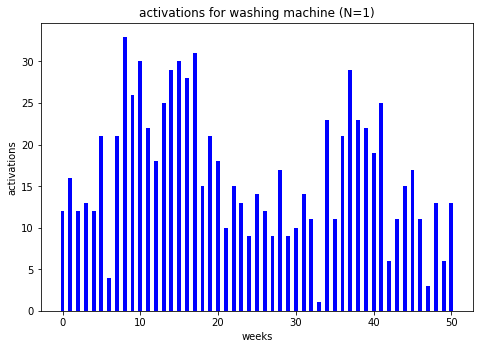
\includegraphics[width=0.8\textwidth]{../Figures/LPS/WM_yearly.png}
	\label{fig:WM_yearly}
\end{figure}

\subsection{Two-dimensional time per-appliance load profiles}

Using a combination of figures \ref{fig:WM_daily} and \ref{fig:WM_weekly},
it is possible to generate a heatmap \ref{fig:wm_hm_weekly}.

\begin{figure}[H]
	\centering
	\caption{"Two-dimensional time per-appliance load profile"}
	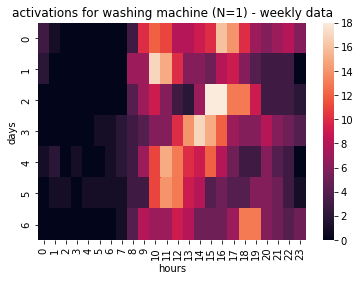
\includegraphics[width=0.7\textwidth]{../Figures/LPS/wm_hm_weekly.png}
	\label{fig:wm_hm_weekly}
\end{figure}

In this case, a similar use case could be fitted as in the first example.
The first example used load shedding for when the demand is too high.
On the contrary, it can also occur the grid demand is too low.
There are two solutions to this issue.
The first one is to decrease production, which can be slow and expensive.
The second option is to load the grid, which can be done in many ways.
One of the ways is to turn on appliances using a control system or notify users to turn on appliances that they have commonly used at that time in the past. 
Due to the increasing percentage of renewable energy sources, more and more energy peaks will be weather dependent such as wind and cloud coverage.
By combining weekly wind forecast, weekly cloud coverage, and users consumption profiles energy providers could notify users to turn on the appliances at peak usage times.

By analyzing figure \ref{fig:wm_hm_weekly} it is possible to see that the user uses a washing machine,
on Wednesdays from  15 to 16 o clock quite commonly. 
Should weather reports indicate high production peaks, the electrical provider should offer low-cost energy for that time of day for all users with similar usage patterns. 
This could all be automated for appliances such as home grid batteries, water heaters, EVs, or even fridges with a control system.
This would mean that operator or electrical distribution company could regulate the demand instantly.
By using load profiles it could prioritize appliances that would be used anyway, which would leave minimal impact on users' routines. 
While renewable energy is cheap to produce, it is expensive to store.
Increased adoption of such resources will require a large amount of energy to be stored and released, this process is at best 80 \% efficient.
If that energy is optimally distributed, less energy would be lost due to conversion.

\subsubsection{Other two-dimensional presentations}

The figures below show how some appliances have a constant usage pattern 
over a year, whereas again others change it. Examples below are randomly picked appliances
from UK-DALE and REFIT. 

\begin{figure}[H]
	\begin{subfigure}{.32\textwidth}
		\centering
		\caption{"Computer"}
		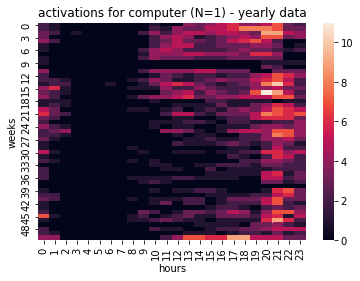
\includegraphics[width=0.9\textwidth]{../Figures/LPS/HM_Ywh_comp.png}
		\label{fig:HM_Ywh_comp}
	\end{subfigure}%
	\begin{subfigure}{.32\textwidth}
		\centering
		\caption{"TV"}
		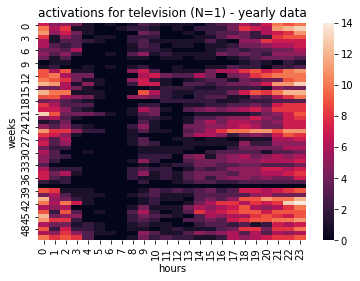
\includegraphics[width=0.9\textwidth]{../Figures/LPS/HM_Ywh_tv.png}
		\label{fig:HM_Ywh_tv}
	\end{subfigure}%
	\begin{subfigure}{.32\textwidth}
		\centering
		\caption{"Washing machine"}
		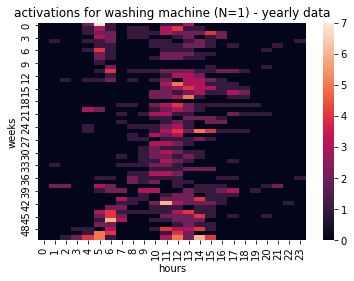
\includegraphics[width=0.9\textwidth]{../Figures/LPS/HM_Ywh_wm.png}
		\label{fig:HM_Ywh_wm}
	\end{subfigure}%
	\caption{Various yearly two-dimensional load profile}
\end{figure}

Another example worth mentioning is one from UK-DALE building 1, where data was collected from 2012-11-09 to 2017-04-26.
Roughly 5 years of data mean that it is possible to build a decent profile. 

\begin{figure}[H]
	\begin{subfigure}{.5\textwidth}
		\centering
		\caption{"solar thermal pumping station"}
		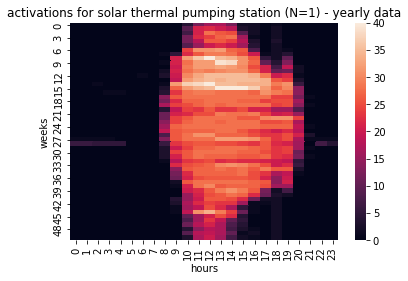
\includegraphics[width=0.9\textwidth]{../Figures/LPS/solar termal pumping station.png}
		\label{fig:solar thermal pumping station}
	\end{subfigure}%
	\begin{subfigure}{.5\textwidth}
		\centering
		\caption{"light"}
		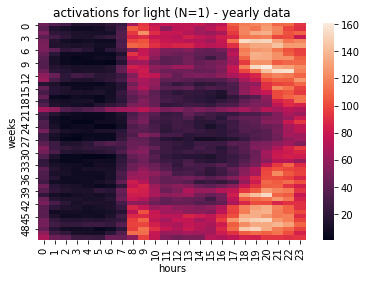
\includegraphics[width=0.9\textwidth]{../Figures/LPS/light.png}
		\label{fig:light}
	\end{subfigure}%
	\caption{"Effect of seasonal changes on load profiles"}
\end{figure}

Figures \ref{fig:solar thermal pumping station} and \ref{fig:light} 
show how weather and season affect the usage pattern of appliances.


\section{Per-house per-appliance}

The last group of profiles is a combination of per-house and per-appliance load profiles.
Observing the usage pattern of many appliances offers a better look into users' usage patterns.
In the case of elderly care, the goal is to observe a group of appliances.
Activation of a group of appliances would yield a contextual event.
If stove and kettle are commonly used together each morning this use could translate to an event such as breakfast. 
In order to achieve this, one needs to observe all appliances at once such as shown on figure \ref{fig:PHPA}.

The figure is also a good example of elderly care system, that would detect an anomaly such as fall, or person unable to get up from the bed in the morning.
This profile shows that first thing in the morning used are kettle and toaster, and with delay of one hour, microwave and TV. 
This enables us to construct time thresholds in which appliances should be used.
If none of these appliances are activated between set thresholds, morning would be considered anomalous.
Although less likely, issues could also occur during the use of appliance. 
In case elder falls during cooking, toasting bread or opening fridge the duty cycle would increase, which would also be considered an anomaly.
In case any of these anomalies are detected, the caregiver would be notified to check on the elder. 

\begin{figure}[H]
	\centering
	\caption{"Daily per-appliance per-house building load profile"}
	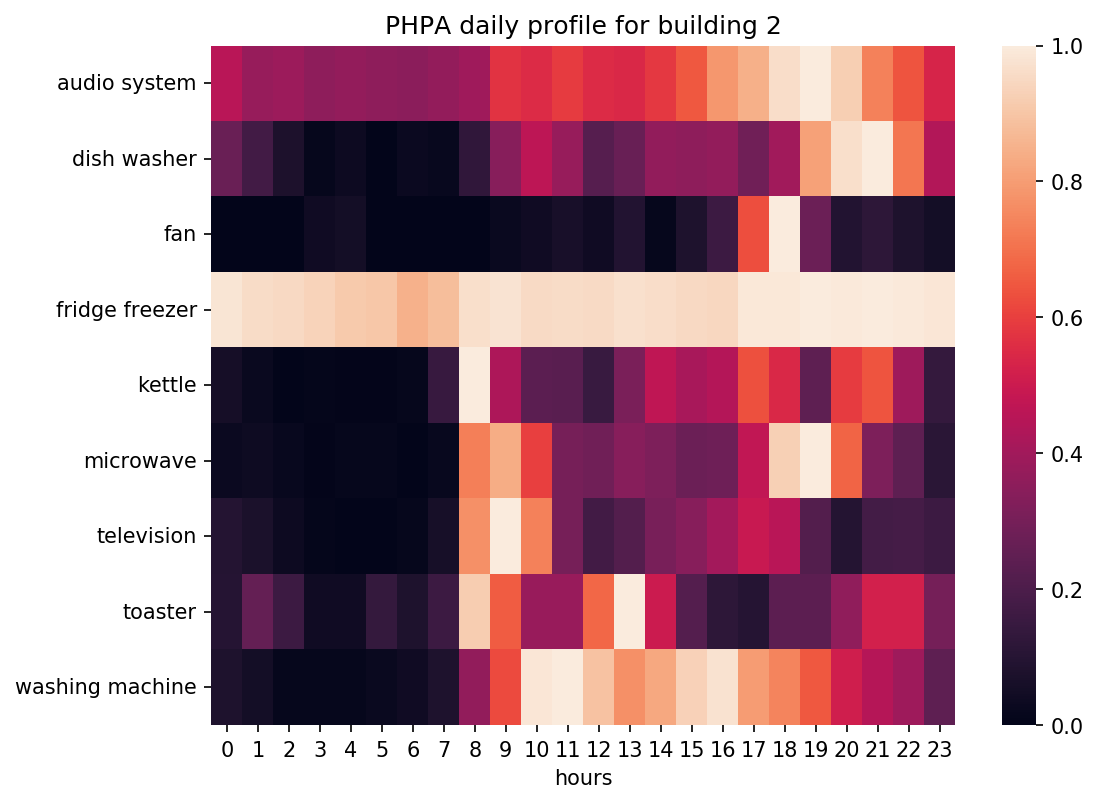
\includegraphics[width=0.7\textwidth]{../Figures/LPS/PHPA.png}
	\label{fig:PHPA}
\end{figure}

The very same data can be presented in an alternative way, such as shown in figure \ref{fig:stack}.
The usage pattern is the same as on \ref{fig:SLPdaily2}, except that it is possible to see
the contribution of each appliance. 

\begin{figure}[H]
	\centering
	\caption{"Stacked daily per-appliance per-house building load profile"}
	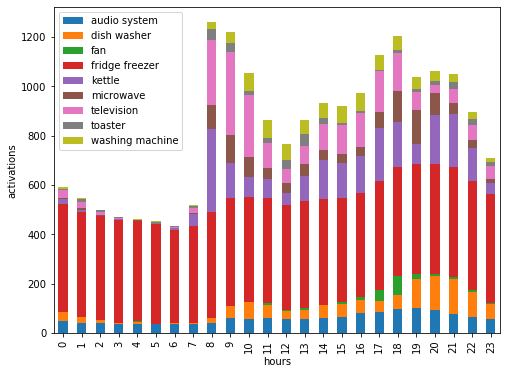
\includegraphics[width=0.7\textwidth]{../Figures/LPS/stack.png}
	\label{fig:stack}
\end{figure}

These load profiles are useful when it comes to analyzing the usage pattern in one building.
In order to be able to process the load-profiles a cross many buildings a new profile must be introduced.
The idea is derived from the bag-of-words method used in text processing, where a list of most commonly used words is formed, and then used to process the text. 
Here, It is possible to use the activation data from all five datasets.
A list of appliances is sorted by number of activations and then only top 30 appliances are selected.
Using this list it is possible to present the usage of each building universally.

\begin{figure}[H]
	\centering
	\caption{"Universal presentation of per-house per-appliance load profile"}
	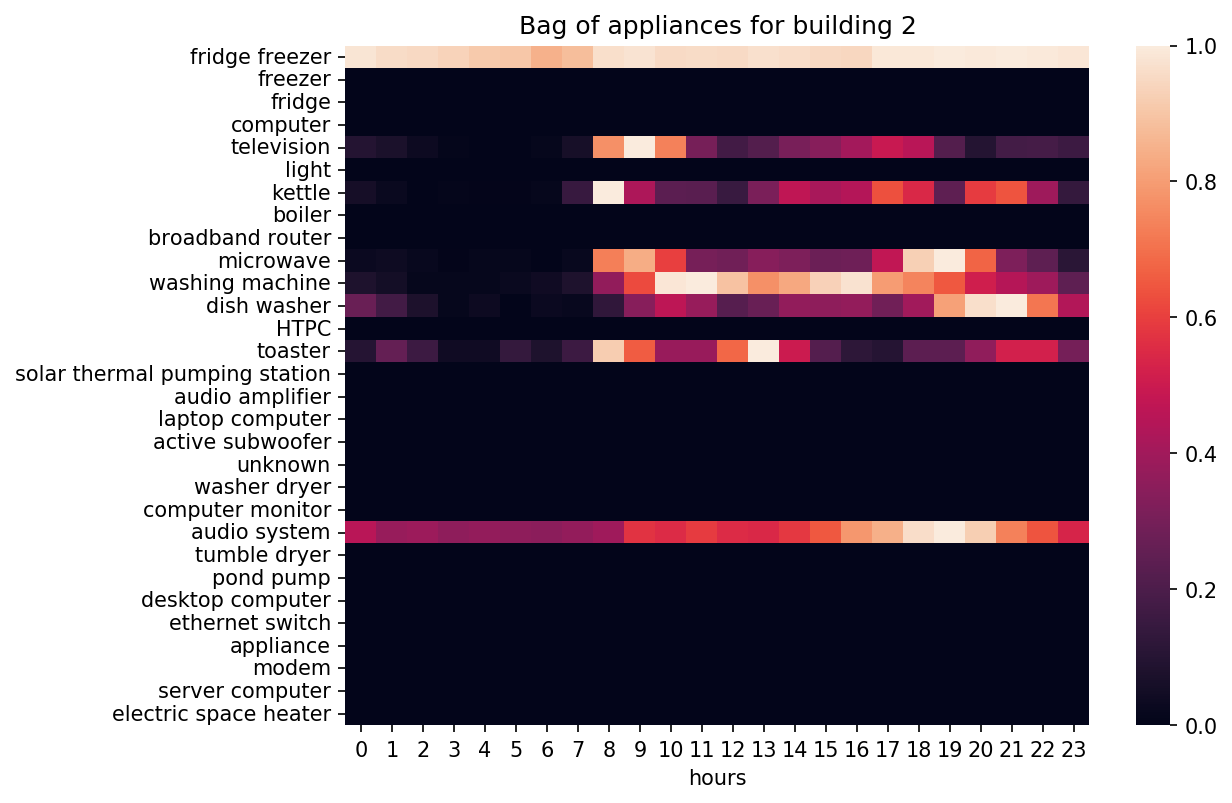
\includegraphics[width=1\textwidth]{../Figures/LPS/BOA.png}
	\label{fig:BOA}
\end{figure}

